\chapter{Code Style}
Voor de code style worden de standaard code style settings van IntelliJ IDEA gebruikt.
De code style wordt ook gecontroleerd door Codacy, een code analyse tool.
Codacy controleert je Java (en Javascript) codebase op verschillende errors.

\begin{figure}[H]
	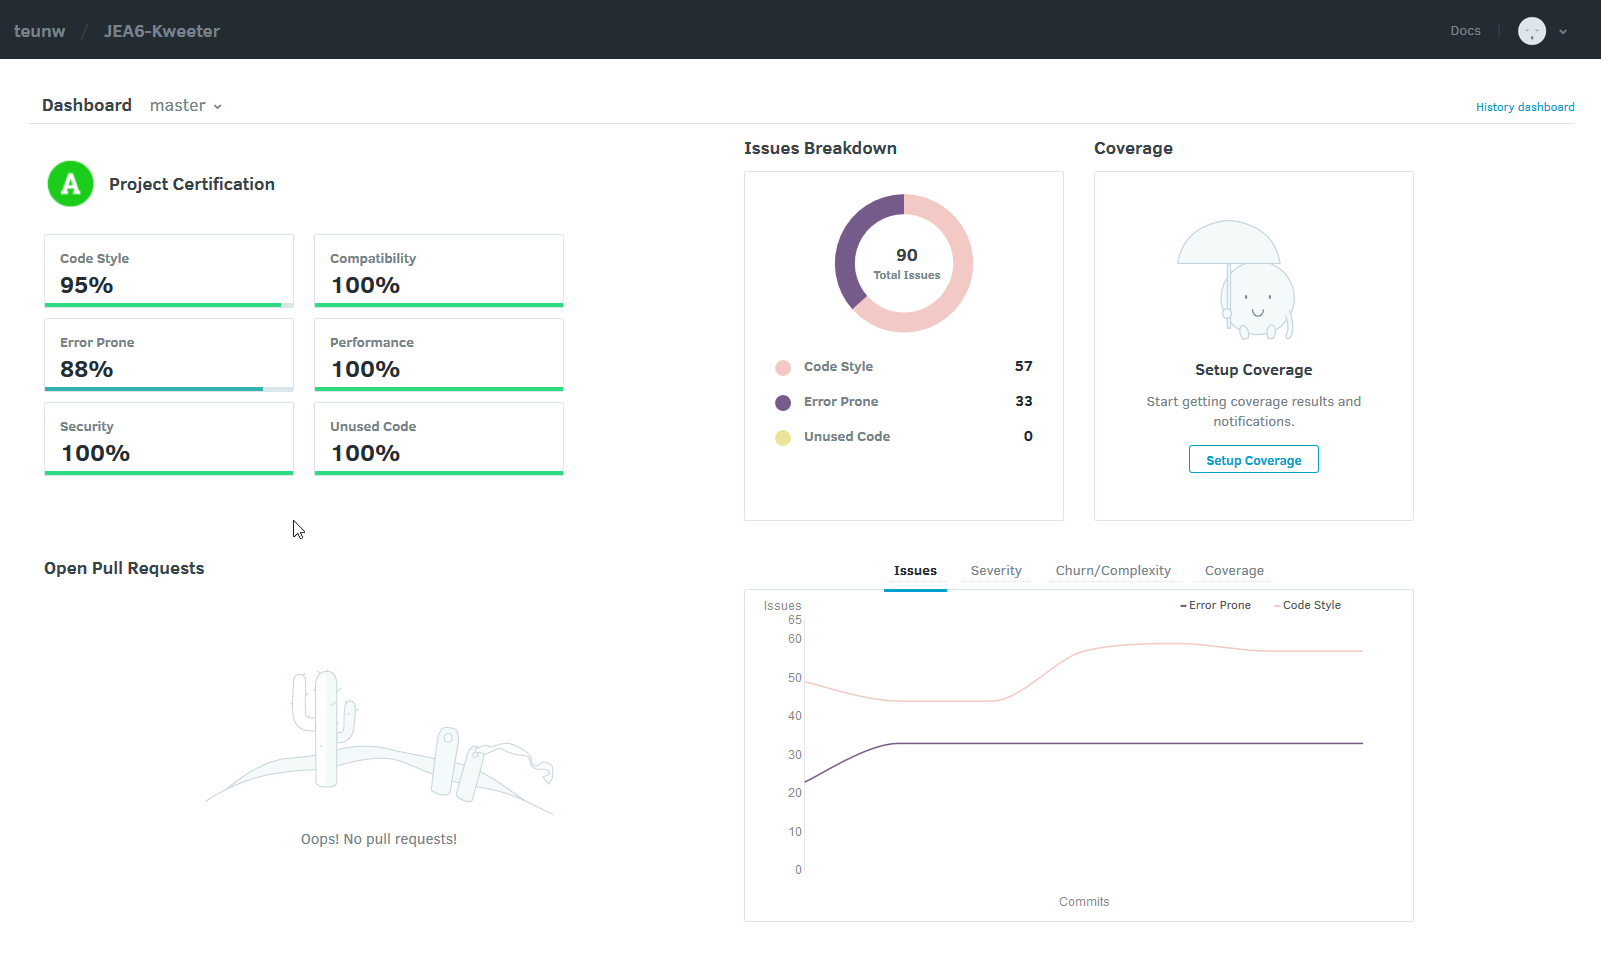
\includegraphics[width=0.75\textwidth]{images/StaticCodeAnalysis.png}
	\caption{Voorbeeld van code analysis door middel van Codacy}
	\label{fig:StaticCodeAnalyses}
\end{figure}

Ook kan er gecontroleerd worden op beveiligingsproblemen in je applicatie, stel dat je bijvoorbeeld SQL-query parameters in je queries hebt staan, dan wordt dat netjes gerapporteerd.
Andere dingen waartegen je beschermt wordt zijn:
\begin{itemize}
	\setlength\itemsep{0em}
	\item Authentication
	\item CSRF aanvallen
	\item File access
	\item SQL Injection
	\item XSS
\end{itemize}

Natuurlijk bied Codacy ook een gedetaileerd overzicht van de verschillende fouten in je code.
\begin{figure}[H]
	\centering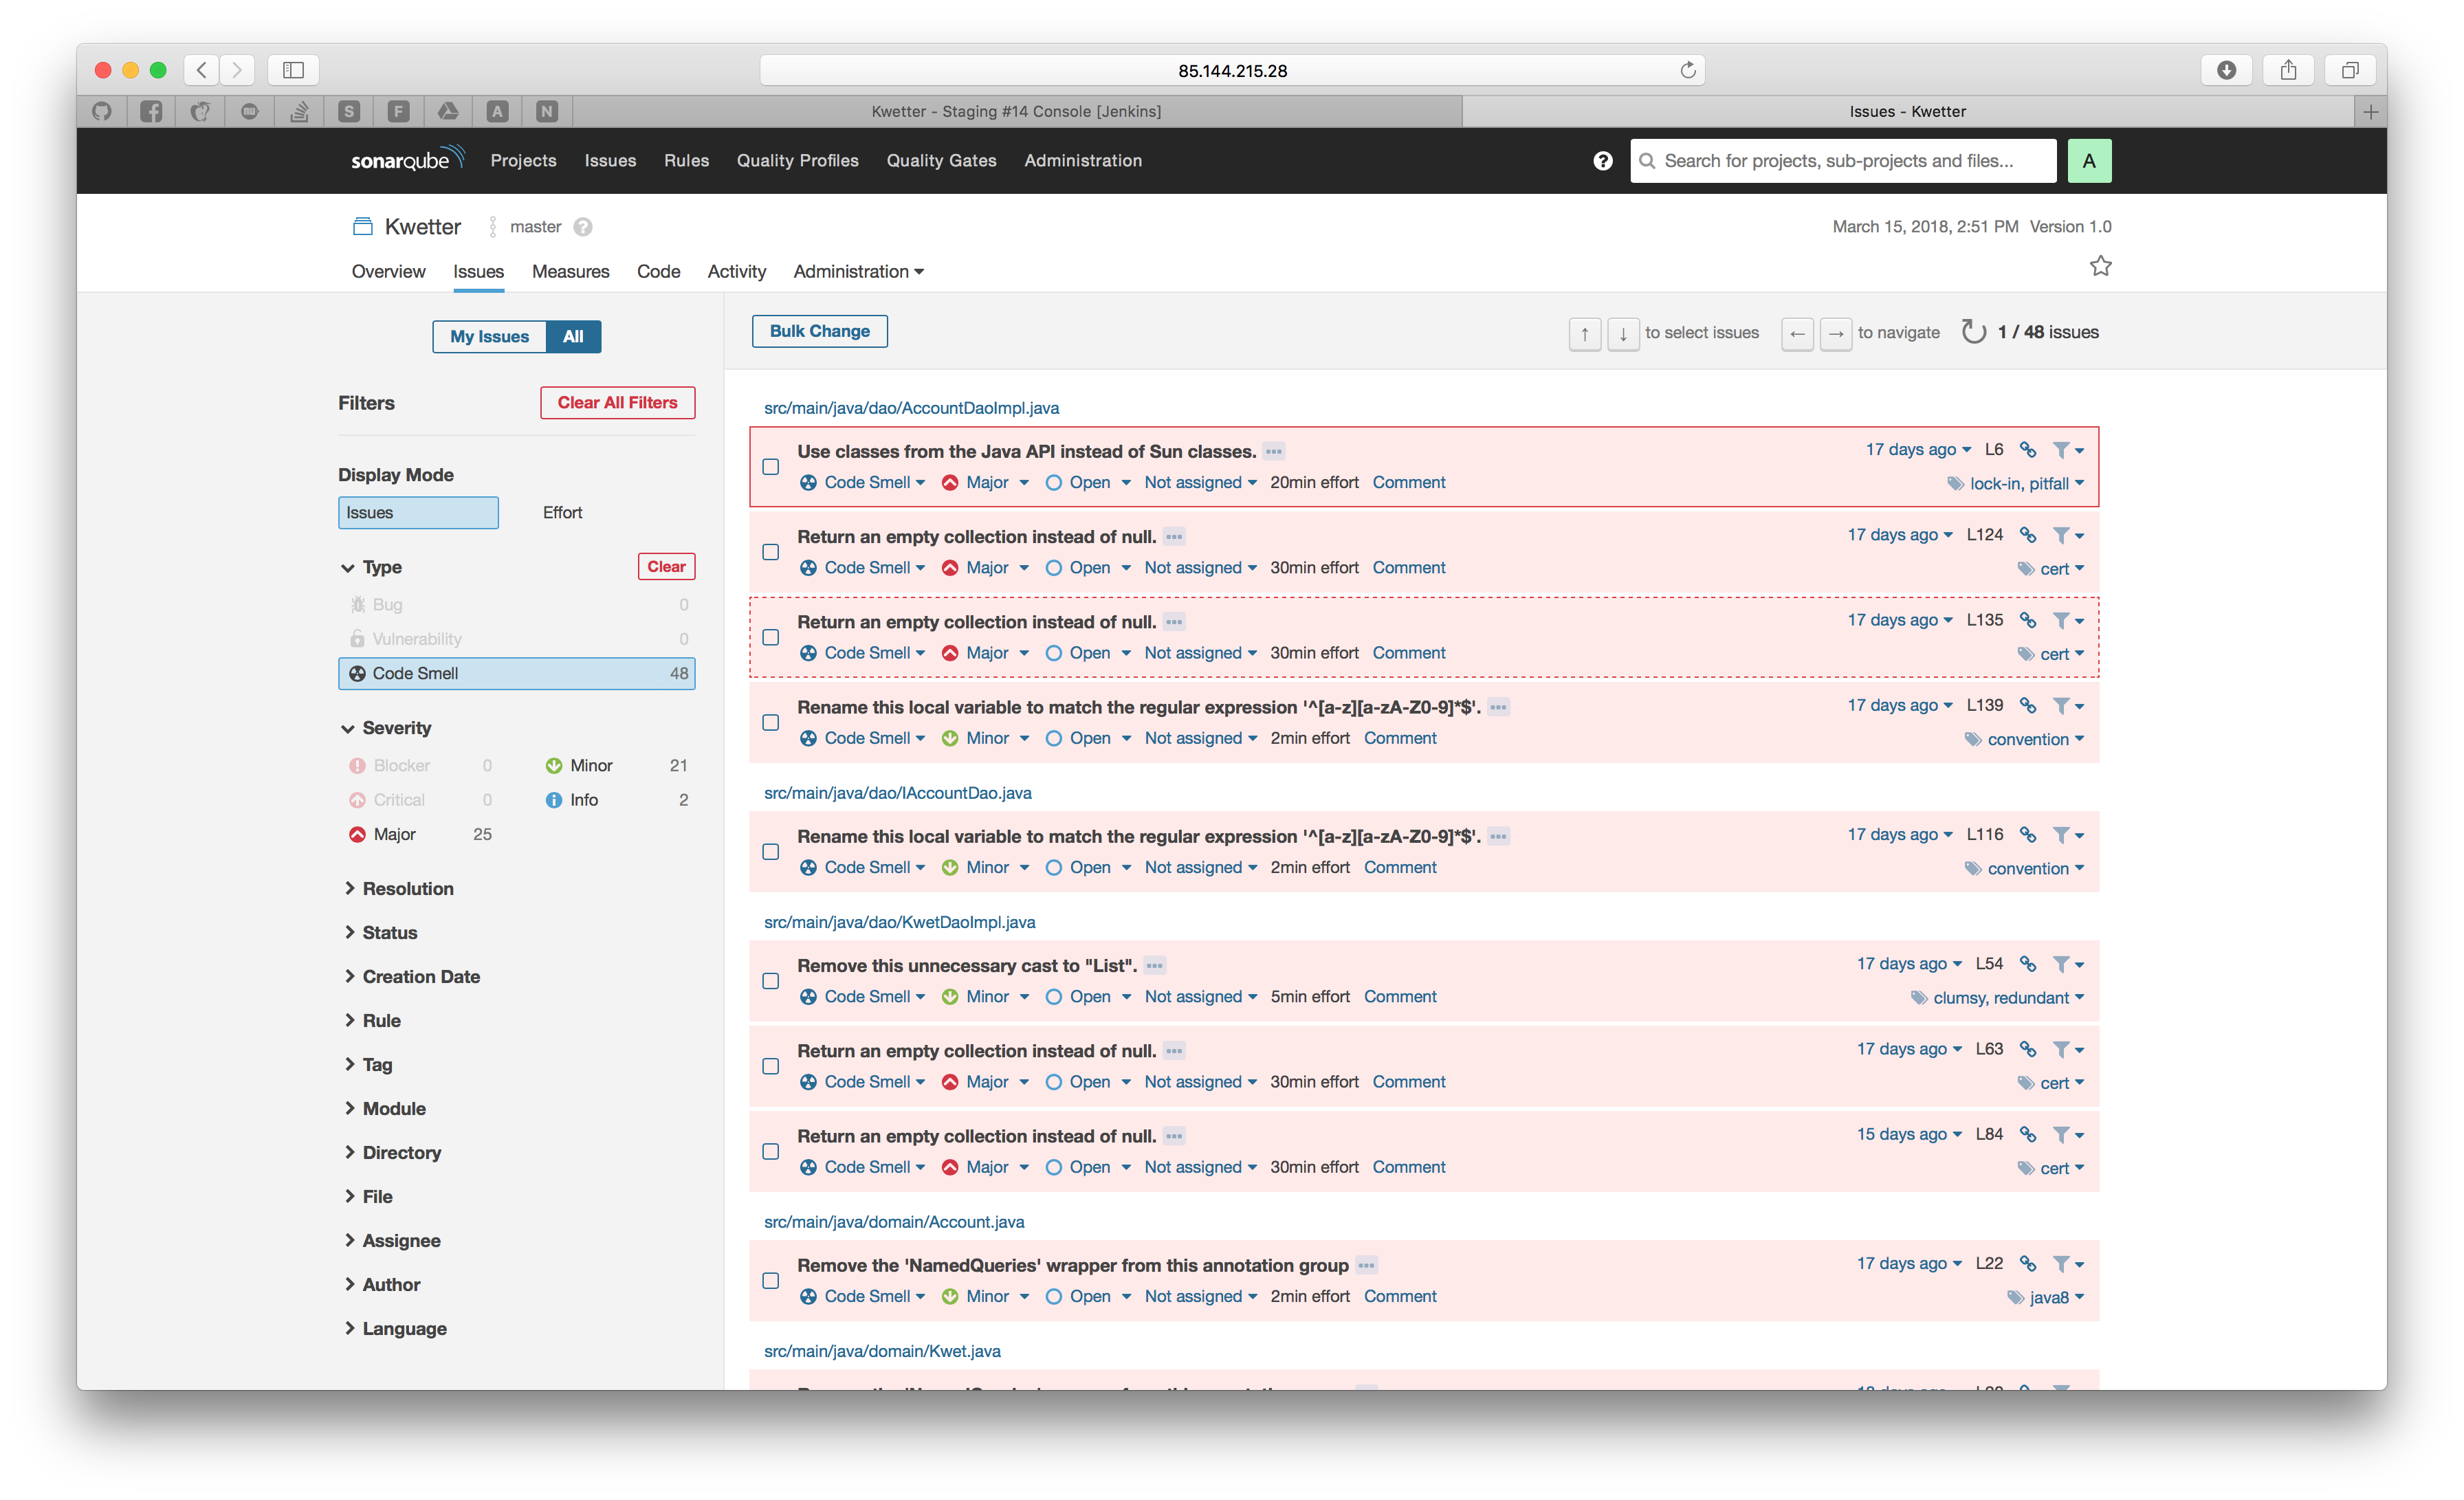
\includegraphics[width=0.5\textwidth]{images/Codacy}
	\caption{Verschillende fouten in een Typescript bestand}
\end{figure}